\documentclass{article}
\usepackage[utf8]{inputenc}
\usepackage{cmap}					% поиск в PDF
\usepackage{mathtext} 				% русские буквы в формулах
\usepackage[T2A]{fontenc}			% кодировка
\usepackage[utf8]{inputenc}			% кодировка исходного текста
\usepackage[english,russian]{babel}	% локализация и переносы
\usepackage{indentfirst}
\documentclass{article}
\usepackage{graphicx}
\graphicspath{ {./images/} }

\title{Отчёт по 4 лабе}
\date{October 2022}

\begin{document}

\maketitle

\section{Описание проектируемого ПО}
\section{Построенные диаграммы моделей}
\section{Анализ недостатков и свойств}

\newpage
\huge {Описание проектируемого ПО} \\ \\
\large{TIA (Turtle Invest Advisor) — Telegram бот для инвестирования, основной идеей которого является использование стратегии усреднения. Стратегия позволяет долгосрочному инвестору получить максимально диверсифицированный портфель. TIA предлагает пользователю рекомендации по покупке определённого количества ценных бумаг по порядку.}

\newpage
\huge{Построенные диаграммы моделей}

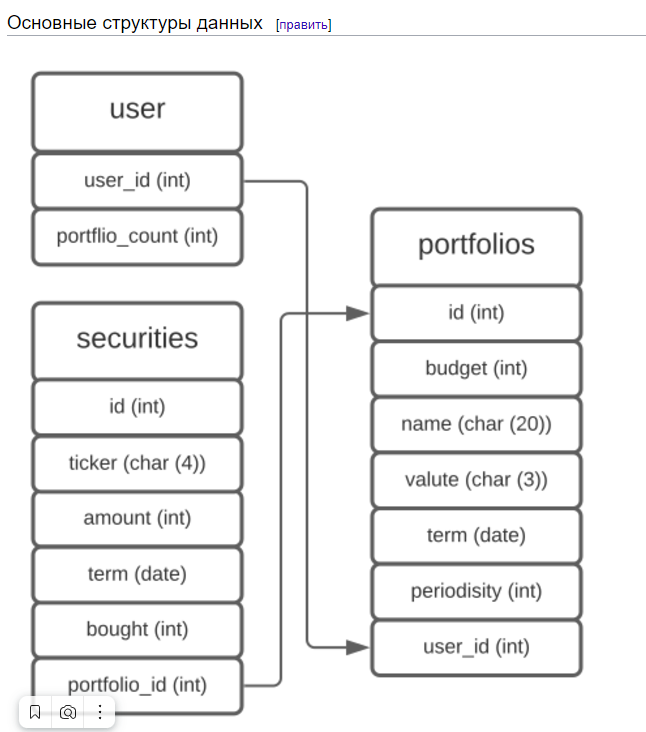
\includegraphics[scale=0.5]{бд.png} \\
\includegraphics[scale=0.7]{моделька.jpg}
\includegraphics[scale=0.5]{modelmydemn.png}

\newpage
\huge{Анализ недостатков и свойств нашего проектирования} \\ \\
\Large{Недостатки} \\ \\
\large{• Не подразумевает далеко идущих планов, например план \\ продаж} \\
\large{• Существование проекта не очень долгое - возможно система не расмотрена с какой-то стороны проектирования}
\\ \\
\Large{Свойства} \\ \\
\large{• Продуманное проектирование - нет исправлений, есть \\ качество} \\
\large{• Наше проектирование допускает отлаженное написание кода} \\

\end{document}
